% Description: Contains the software state of the art.

\section{Software}
In this section, we will discuss all software-related topics researched for the development of this project. Topics include flight controller firmware, ground control stations, companion computer operating systems, ROS 2 documentation, computer vision, ArUco markers, and others.

\subsection{FC Firmware}
The definition of firmware, according to the \textit{ISO/IEEE}, is \textit{“combination of a hardware device and computer instructions and data that reside as read-only software on that device”} \cite{iso_firmware}. For flight controllers, firmware is the software that runs on the flight controller and is responsible for managing the sensors, actuators, and control algorithms required to maintain the stability and control of the vehicle.

Several flight controller firmware options are available today, each with its unique characteristics and advantages. In this project, two of the most popular and widely used firmware in the drone and unmanned vehicle industry were investigated: PX4 and ArduPilot.

\subsubsection{PX4 Firmware}
PX4 firmware has been a fundamental component in the development of flight control systems for drones and unmanned vehicles, standing out for its open-source nature and flexibility for many applications. According to the official documentation, \textit{``PX4 is a powerful open source autopilot flight stack running on the NuttX RTOS''} \cite{px4_docs}. This system is widely recognized for its modular architecture, which allows the integration of new sensors, actuators, and control algorithms, enabling specific adaptations to meet the requirements of different projects \cite{px4_docs}.

Among its most notable features is its ability to support a wide variety of vehicle types. In this regard, PX4 \textit{``supports many different vehicle frames/types, including: multicopters, fixed-wing aircraft (planes), VTOLs (hybrid multicopter/fixed-wing), ground vehicles, and underwater vehicles''} \cite{px4_docs}. This multi-configuration capability is essential, as it allows the same framework to be applied to various platforms with minimal modifications.

Additionally, PX4 is an integral part of a broader ecosystem that includes ground control stations such as QGroundControl, Mission Planner, and specific hardware like Pixhawk. The documentation mentions that \textit{``PX4 is a core part of a broader drone platform that includes the QGroundControl ground station, Pixhawk hardware, and MAVSDK for integration with companion computers, cameras, and other hardware using the MAVLink protocol''} \cite{px4_docs}. This integration ensures seamless communication between the different system components, which is crucial for real-time monitoring and mission planning.

Finally, PX4 offers \textit{``flexible and powerful flight modes and safety features''}, which are vital for projects requiring complex maneuvers, such as precise autonomous landing on charging stations \cite{px4_docs}. These advanced control functionalities and its ability to integrate with computer vision technologies and external sensors establish PX4 as a key tool in the development of high-relevance autonomous vehicle technologies.

\subsubsection{ArduPilot Firmware}
ArduPilot, like PX4, is open-source software that runs on a wide variety of hardware, allowing the creation and use of autonomous systems for unmanned vehicles in different applications. According to the official documentation, \textit{“ArduPilot provides a comprehensive suite of tools suitable for almost any vehicle and application. As an open source project, it is constantly evolving based on rapid feedback from a large community of users”} \cite{ardupilot_docs}. This flexibility and adaptability have made ArduPilot an essential tool for automation and robotics projects seeking a versatile and robust solution.

One of the most notable aspects of ArduPilot is that, unlike PX4, it does not manufacture hardware. Instead, \textit{“ArduPilot firmware works on a wide variety of different hardware to control unmanned vehicles of all types”} \cite{ardupilot_docs}. This means it can integrate with different types of controllers, sensors, and devices, transforming virtually any mobile machine into an autonomous vehicle with the simple addition of an appropriate hardware package.

As mentioned earlier, firmware is the code that runs on the controller, and the choice of firmware depends on the vehicle and mission. As stated in the documentation, \textit{“You choose the firmware to match your vehicle and mission: Copter, Plane, Rover, Sub, or Antenna Tracker”} \cite{ardupilot_docs}. This versatility allows developers to select the configuration most appropriate for their specific needs, optimizing the development and operation process.

ArduPilot is also complemented by ground control stations (GCS), which function as the interface between the user and the vehicle's controller. One of the most comprehensive tools in this area is Mission Planner, described as \textit{“a full-featured GCS supported by ArduPilot”}, offering easy and fast interaction with the firmware \cite{ardupilot_docs}.

Lastly, it is worth mentioning that both PX4 and ArduPilot share similar functionalities such as sensor calibration, mission planning, parameter configuration, among others. However, the choice between the two will depend on the specific needs of the project and the compatibility with the available \textbf{hardware}.

\subsection{Ground Control Systems (GCS)}
Ground control systems (GCS) are auxiliary tools widely used for the configuration, calibration, and monitoring of drones. Although they are not the main focus of this project, they play an important role in system preparation, facilitating parameter configuration, sensor calibration, and supervision during test flights.

Among the tools used are QGroundControl and Mission Planner, which stand out for their compatibility with PX4 and ArduPilot firmware, respectively. These platforms provide intuitive interfaces for adjusting vehicle parameters, planning missions, and visualizing real-time telemetry data. In the context of this project, they have been key to ensuring that the drone is properly configured before being integrated with the modular charging station.

Despite their usefulness during the preparation and testing stages, the proposed system does not directly rely on these tools for its final operation. The autonomous operation of the drone and the charging station is based on direct interaction between the firmware, vision systems, and flight controllers, without requiring continuous intervention from a ground control station.

\begin{figure}[h!]
    \centering
    \begin{subfigure}{0.48\textwidth}
        \centering
        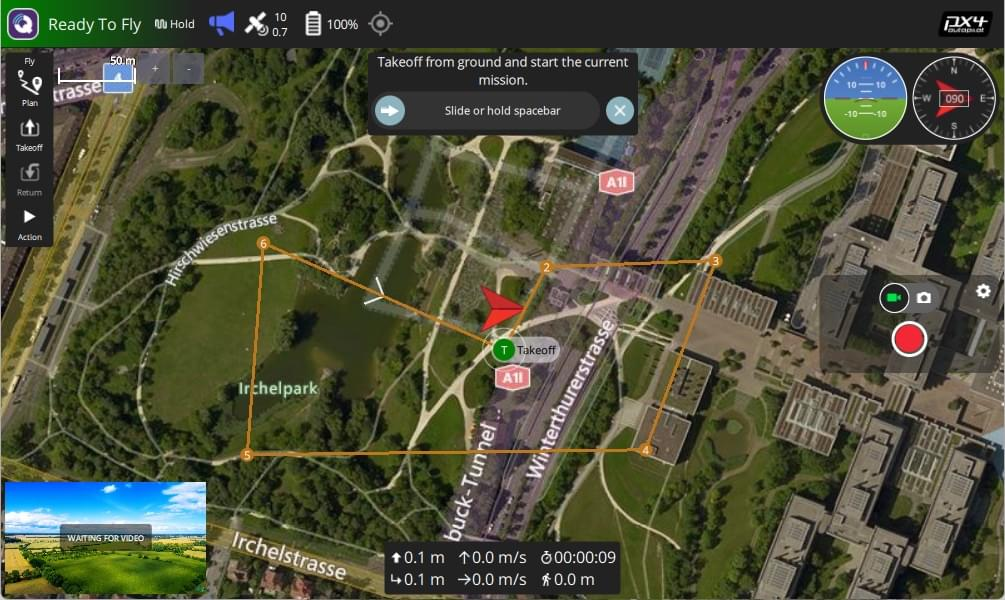
\includegraphics[width=\textwidth]{pictures/qgc_interface.jpg} % Illustrative image of QGroundControl
        \caption{QGroundControl Interface.}
        \label{fig:qgc}
    \end{subfigure}
    \hfill
    \begin{subfigure}{0.48\textwidth}
        \centering
        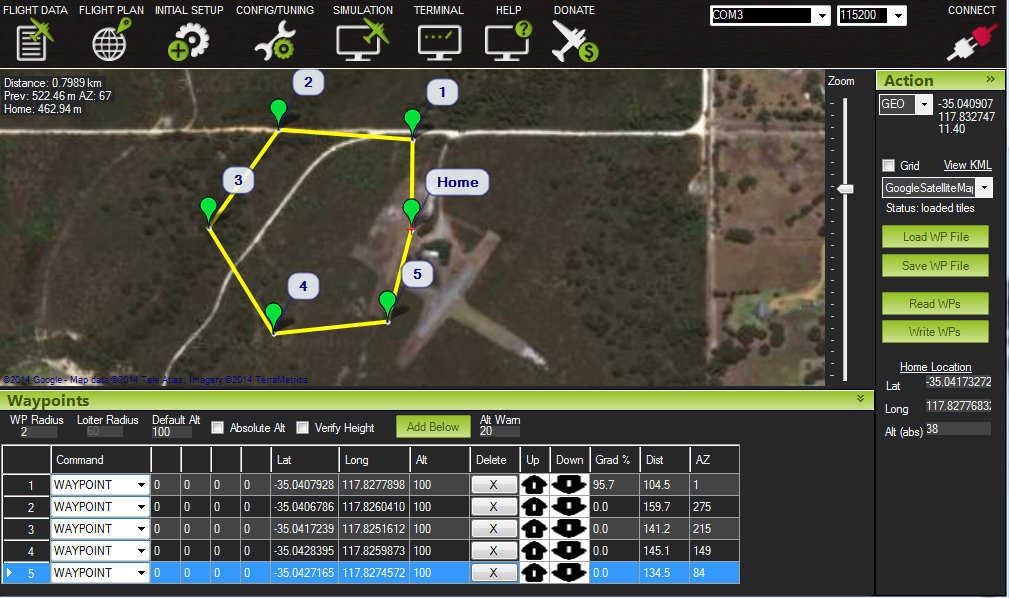
\includegraphics[width=\textwidth]{pictures/mission_planner.jpg} % Illustrative image of Mission Planner
        \caption{Mission Planner Interface.}
        \label{fig:mission_planner}
    \end{subfigure}
    \caption{Ground Control Systems used during configuration and testing stages.}
    \label{fig:gcs}
\end{figure}



\subsection{Operative Systems} 

To operate a companion computer, it is necessary to choose from the many available operating systems, with Ubuntu and Raspberry Pi OS being among the most popular options. Below, the features and advantages of each operating system are described.

\subsubsection{Ubuntu}

Ubuntu is an open-source operating system based on Linux, widely recognized for its stability and large support community. It is important to note that within Ubuntu and its versions, even-numbered releases are more stable. According to Ubuntu's official documentation, this system is \textit{“designed for security, reliability, and ease of use”} \cite{ubuntu_docs}. In the context of companion computers for drones and other autonomous vehicles, Ubuntu is frequently used due to its compatibility with robotics tools such as ROS (Robot Operating System), facilitating the integration and development of advanced software for control and automation.

Ubuntu supports ARM architectures, allowing its installation and operation on devices such as Raspberry Pi 4 and 5. This capability is essential for projects that require efficient local processing, sensor data handling, and real-time communication. Additionally, Ubuntu's flexibility allows for its environment to be customized to meet the specific needs of the project, whether for running flight control nodes or real-time image processing \cite{ubuntu_docs}.

\subsubsection{Raspberry Pi OS}

Raspberry Pi OS is the official operating system developed and optimized for Raspberry Pi devices. The Raspberry Pi OS documentation describes it as \textit{“a Debian-based operating system specifically tuned for the Raspberry Pi hardware”} \cite{raspbian_docs}. Its main advantage is its optimization for Raspberry Pi hardware, ensuring optimal performance and efficient use of available resources.

Raspbian includes a series of pre-installed tools that facilitate development and prototyping, making it a preferred option for educational and research projects. Its compatibility with Python and other programming libraries makes it easier to implement scripts and software necessary for many robotics applications.

Compared to other operating systems, Raspbian is lightweight and allows for a \textbf{quick boot}, which is beneficial in scenarios where the system needs to start quickly.


\subsection{ROS2 Distributions}

The ROS 2 (Robot Operating System 2) distributions provide standardized environments for the development of robotic applications, each tailored to different needs and hardware capabilities. One of the advantages of ROS 2 is its ability to \textbf{facilitate cross-distribution communication} through the use of topics, allowing nodes in different ROS 2 versions to communicate and collaborate effectively within the same project \cite{ros_docs}. The following sections provide details about the most recent and stable ROS 2 distributions.

\subsubsection{Humble Distribution}

The \textbf{ROS 2 Humble Hawksbill} distribution is known for being a version with \textbf{long-term support (LTS)}, which guarantees consistent and reliable updates. This distribution is designed for projects requiring stability and high compatibility with different systems and packages. It is ideal for hardware such as the \textbf{Raspberry Pi 4} and is compatible with \textbf{Ubuntu 22.04} and earlier versions like Ubuntu 20.04, making it accessible for more standard hardware configurations.

According to the official ROS 2 documentation, Humble is one of the most recommended versions for projects seeking long-term consistency due to its focus on avoiding disruptive changes \cite{humble_documentation}.

\paragraph{Key Features:}
\begin{itemize}
    \item \textbf{LTS (Long-Term Support):} Ensures extended support for updates and bug fixes.
    \item \textbf{Stability:} Proven improvements in node communication, ensuring reliability.
    \item \textbf{Broad compatibility:} Works with most libraries and packages within the ROS 2 ecosystem.
    \item \textbf{Optimized for ARM:} Ideal for platforms like the Raspberry Pi 4, efficiently utilizing limited resources.
\end{itemize}

Overall, Humble is the preferred choice for those prioritizing stability in research projects or long-term applications.

\subsubsection{Jazzy Distribution}

The \textbf{ROS 2 Jazzy Jalisco} distribution, newer than Humble, is designed to take advantage of modern hardware like the \textbf{Raspberry Pi 5} and is compatible with advanced operating systems such as \textbf{Ubuntu 24.04}. This distribution includes significant performance improvements and new functionalities but is considered more experimental compared to LTS versions.

According to Jazzy's documentation, its primary focus is to facilitate the development of robotic applications that leverage the latest tools and simulators while improving the speed of node-to-node communication \cite{jazzy_documentation}.

\paragraph{Key Features:}
\begin{itemize}
    \item \textbf{New functionalities:} Introduction of experimental features and performance adjustments.
    \item \textbf{Lower latency:} Faster communication between nodes, crucial for real-time applications.
    \item \textbf{Advanced integration:} Improvements in simulation and debugging, leveraging tools like Gazebo and Rviz.
    \item \textbf{Hardware-oriented design:} Designed for devices such as the Raspberry Pi 5, offering greater processing capacity.
\end{itemize}

\begin{figure}[h!]
    \centering
    
\includegraphics[width=0.3\textwidth]{pictures/humble_logo.png}
    \caption{ROS 2 Humble}
    \label{fig:imagen1}
\end{figure}

\begin{figure}[h!]
    \centering
    
\includegraphics[width=0.3\textwidth]{pictures/jazzy_logo.png}
    \caption{ROS 2 Jazzy Jalisco}
    \label{fig:imagen2}
\end{figure}

\subsection{ROS 2 Architecture}

    ROS 2 (Robot Operating System 2) is a set of libraries and tools designed for developing robotics applications. It is the evolution of ROS 1, created to address issues related to scalability, security, and support for real-time systems. ROS 2 uses an architecture based on the middleware \textbf{DDS (Data Distribution Service)}, which facilitates communication between nodes in distributed systems, ensuring interoperability and low response times \cite{ros_docs}.  
    
    \subsubsection{Basic Concepts of ROS 2}
    
    ROS 2 is organized around several fundamental elements that enable interaction between different parts of the robotic system. These elements, which define its modular architecture, are essential for understanding how a system based on ROS 2 is structured and functions \cite{ros_docs}:  
    
    \begin{itemize}
        \item \textbf{Nodes:} These are the basic execution units in ROS 2. Each node performs a specific function, such as collecting data from a sensor or controlling an actuator. Nodes are designed to be independent and communicate with each other through topics, services, or actions.  
        \item \textbf{Messages:} These are data structures sent between nodes to share information. Messages have a defined format that ensures all nodes understand the content.  
        \item \textbf{Topics:} These represent communication channels for exchanging messages between nodes. Communication through topics is asynchronous, allowing nodes to publish and receive information without waiting for immediate responses.  
        \item \textbf{Services:} These enable synchronous communication between nodes. Unlike topics, services operate on a request-and-response model, useful for specific operations.  
        \item \textbf{Actions:} Similar to services, but designed for long-duration operations. They allow nodes to receive updates on the progress of a task and cancel it if necessary.  
        \item \textbf{Launch Files:} These simplify the configuration and simultaneous startup of multiple nodes, facilitating the management of complex applications, especially in distributed environments.  
        \item \textbf{Parameters:} Configurable values that nodes use to adjust their behavior without modifying the code.  
    \end{itemize}
    
    The combination of these elements allows robotic systems designed in ROS 2 to be highly scalable and flexible, adapting to both small projects and complex systems.  
    
    % Image of ROS 2 Architecture
    \begin{figure}[h!]
        \centering
        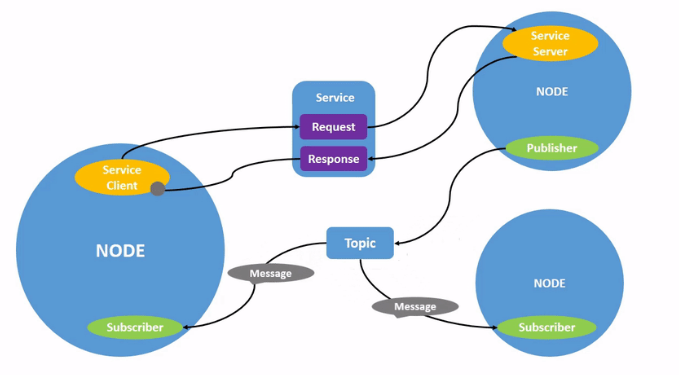
\includegraphics[width=0.6\textwidth]{pictures/ros2_arch.png}
        \caption{ROS 2 Architecture \cite{ros_docs}.}
        \label{fig:ros2_architecture}
    \end{figure}
    
    \subsubsection{Key Benefits of ROS 2}
    
    The architecture of ROS 2 brings several advantages that make it ideal for modern distributed robotic systems. Among the key benefits are the following \cite{ros_docs}:  
    
    \begin{table}[h!]
    \centering
    \caption{Key Benefits of ROS 2}
    \begin{tabular}{|l|p{10cm}|}
    \hline
    \textbf{Benefit} & \textbf{Description} \\
    \hline
    Multithreading & Allows nodes to run in parallel, optimizing performance. \\
    \hline
    Use of topics & Asynchronous communication between nodes for data exchange. \\
    \hline
    Nodes and services & Nodes interact through services and topics for specific tasks. \\
    \hline
    Launch files & Configure and execute multiple nodes simultaneously. \\
    \hline
    Fast communication & Based on DDS, provides low-latency communication between nodes. \\
    \hline
    Custom messages & Enables defining and using specific structures for each application. \\
    \hline
    Real-time support & Enables critical applications where response time is essential. \\
    \hline
    \end{tabular}
    \label{table:benefits}
    \end{table}    

---

\subsection{Computer Vision}

    Computer vision is a programming field that allows systems to interpret and process visual information from the environment. This field is key in applications requiring real-time image and video analysis, such as autonomous robot navigation, object detection, and artificial intelligence systems. To facilitate the development of these applications, specialized tools and libraries such as OpenCV play a fundamental role in the practical implementation of computer vision \cite{opencv_docs}.  
    
    \subsubsection{OpenCV Library}
    
    OpenCV (Open Source Computer Vision Library) is one of the most widely used libraries in industry and academia for developing computer vision solutions. According to its official documentation, OpenCV is \textit{“an open-source computer vision and machine learning software library containing more than 2500 optimized algorithms”} \cite{opencv_docs}. These tools enable tasks such as image processing, object recognition, and motion tracking, and are compatible with programming languages like Python and C++.  
    
    Thanks to its flexibility and ease of use, OpenCV is suitable for both beginners and experts. Moreover, its optimized algorithms enable real-time processes, making it an ideal tool for robotics projects and autonomous applications \cite{opencv_docs}.  
    
    \subsubsection{Camera Calibration}
    
    Before implementing any computer vision system in applications that demand spatial accuracy, it is essential to perform proper camera calibration. This process corrects inherent lens distortions and enables precise measurements of the environment. According to OpenCV documentation, \textit{“Camera calibration is the process of estimating the parameters of the lens and the image sensor of an imaging device”} \cite{opencv_calib3d}.  
    
    Calibration involves determining intrinsic parameters (such as focal length and principal point) and extrinsic parameters (relative to the camera's position and orientation) that map 2D coordinates from captured images to real-world 3D coordinates.  
    
    \begin{figure}[h!] 
        \centering 
        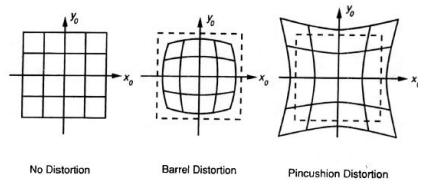
\includegraphics[width=0.6\textwidth]{pictures/distortions.png} % Image of barrel and pincushion distortions inherent to cameras 
        \caption{Types of camera distortions.} 
        \label{fig:distortions} 
    \end{figure}  
    
    OpenCV provides functions that allow this process to be performed efficiently by detecting patterns in images, such as chessboards or circle grids. The typical calibration workflow includes:  
    
    \begin{itemize}
        \item Capturing images of a known pattern from different angles.  
        \item Identifying points of interest in the captured images (pattern corners).  
        \item Using optimization algorithms to calculate intrinsic parameters and distortion coefficients.  
    \end{itemize}  
    
    The result of calibration corrects distortions in images and videos, improving the accuracy of computer vision applications. This is especially useful in projects requiring precise spatial analysis, such as autonomous navigation and real-time object positioning.  
    
    \begin{figure}[h!] 
        \centering 
        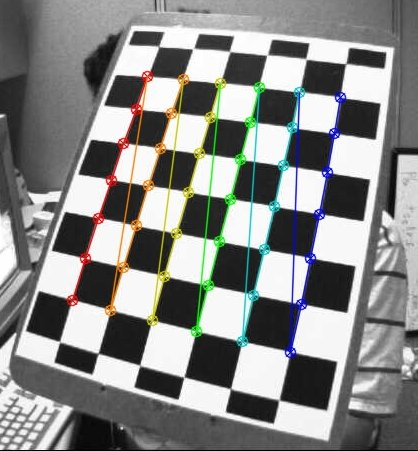
\includegraphics[width=0.4\textwidth]{pictures/calib_pattern.jpg} % Illustrative image of a chessboard used for camera calibration 
        \caption{Chessboard pattern used in camera calibration with OpenCV.} 
        \label{fig:calib_pattern} 
    \end{figure}  


\subsection{What is an ArUco?}
    ArUco, whose name comes from the combination of "Artificial" and "Uco" (for the University of Córdoba, where it was developed), is an open-source library widely recognized in the field of computer vision for detecting fiducial markers in images. This technology is essential for estimating the camera pose relative to the markers when the camera has been previously calibrated. According to the documentation, \textit{“ArUco is an OpenSource library for detecting squared fiducial markers in images”} \cite{aruco_docs}. Detecting these markers is crucial in applications requiring precise estimation of the position and orientation of objects in three-dimensional space.

    \subsubsection{History of ArUco Markers}

    ArUco markers were developed as a solution to overcome the limitations of other technologies for detecting patterns, colors, or shapes. The goal was to create a technique that provides high reliability even under partial occlusions and varying lighting conditions. Early studies focused on the automatic generation of markers with a design that ensured their uniqueness and ease of detection. These markers consist of a binary pattern surrounded by a black border, enhancing their visibility and robustness under different lighting conditions \cite{aruco_docs}.

    \begin{figure}[h!] 
        \centering 
        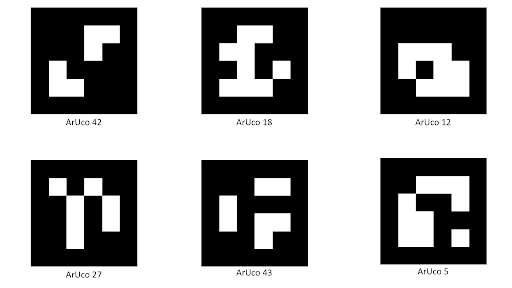
\includegraphics[width=0.8\textwidth]{pictures/arucos_ids.png} % Example of ArUco marker pose detection 
        \caption{Examples of ArUco markers and IDs.} 
        \label{fig} 
    \end{figure}

    \subsubsection{Common Applications}

    ArUco markers are used in various applications, including camera calibration, augmented reality, and robot and drone navigation and control. One of the advantages of using ArUco is their ability to act as reference points in 3D environments, enabling computer vision systems to calculate the camera pose. According to the documentation, \textit{“Markers can be used as 3D landmarks for camera pose estimation”} \cite{aruco_docs_pdf}. This feature makes markers essential in tracking and positioning systems where precision is critical.

    \begin{figure}
        \centering
        \begin{minipage}{0.3\textwidth}
            \centering
            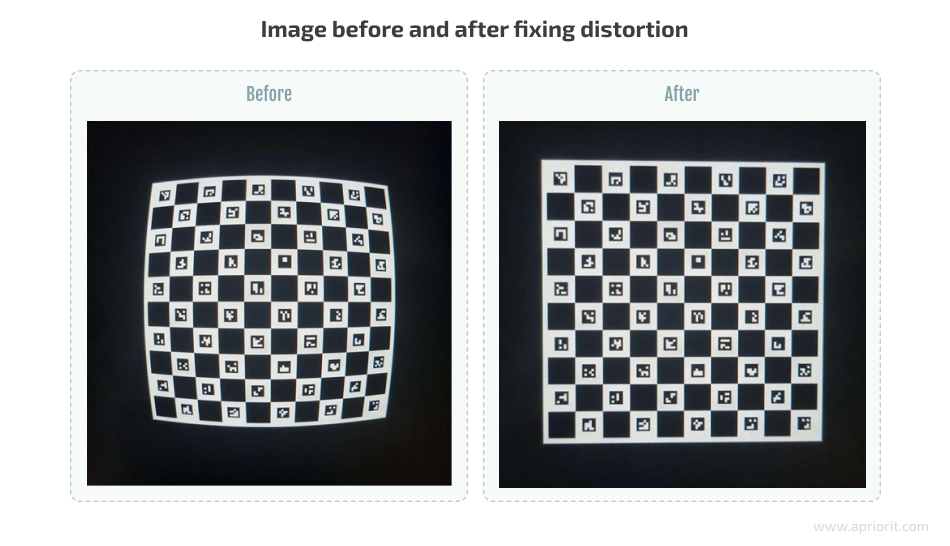
\includegraphics[width=0.8\textwidth]{pictures/calibration_aruco.png}
            \caption{Camera Calibration with ArUco}
            \label{fig:imagen1}
        \end{minipage}
        \hfill
        \begin{minipage}{0.3\textwidth}
            \centering
            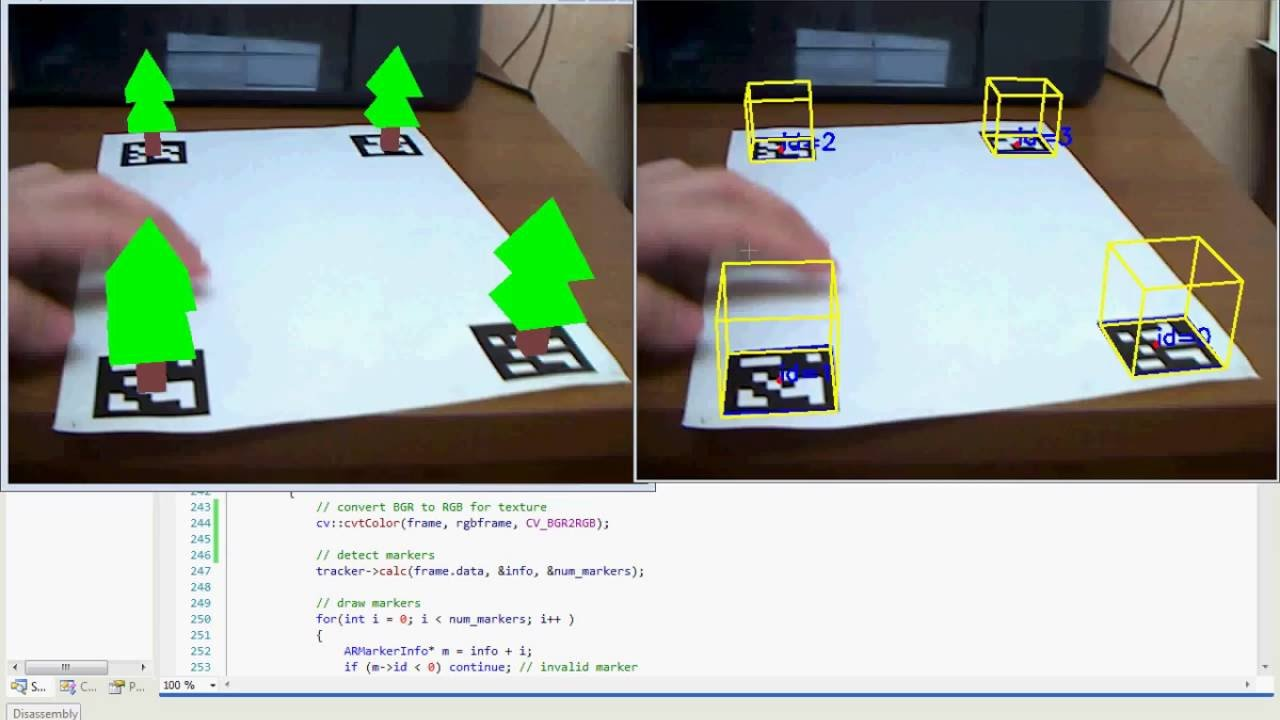
\includegraphics[width=0.8\textwidth]{pictures/augmented_reality.jpg}
            \caption{Augmented Reality with ArUco}
            \label{fig:imagen2}
        \end{minipage}
        \hfill
        \begin{minipage}{0.3\textwidth}
            \centering
            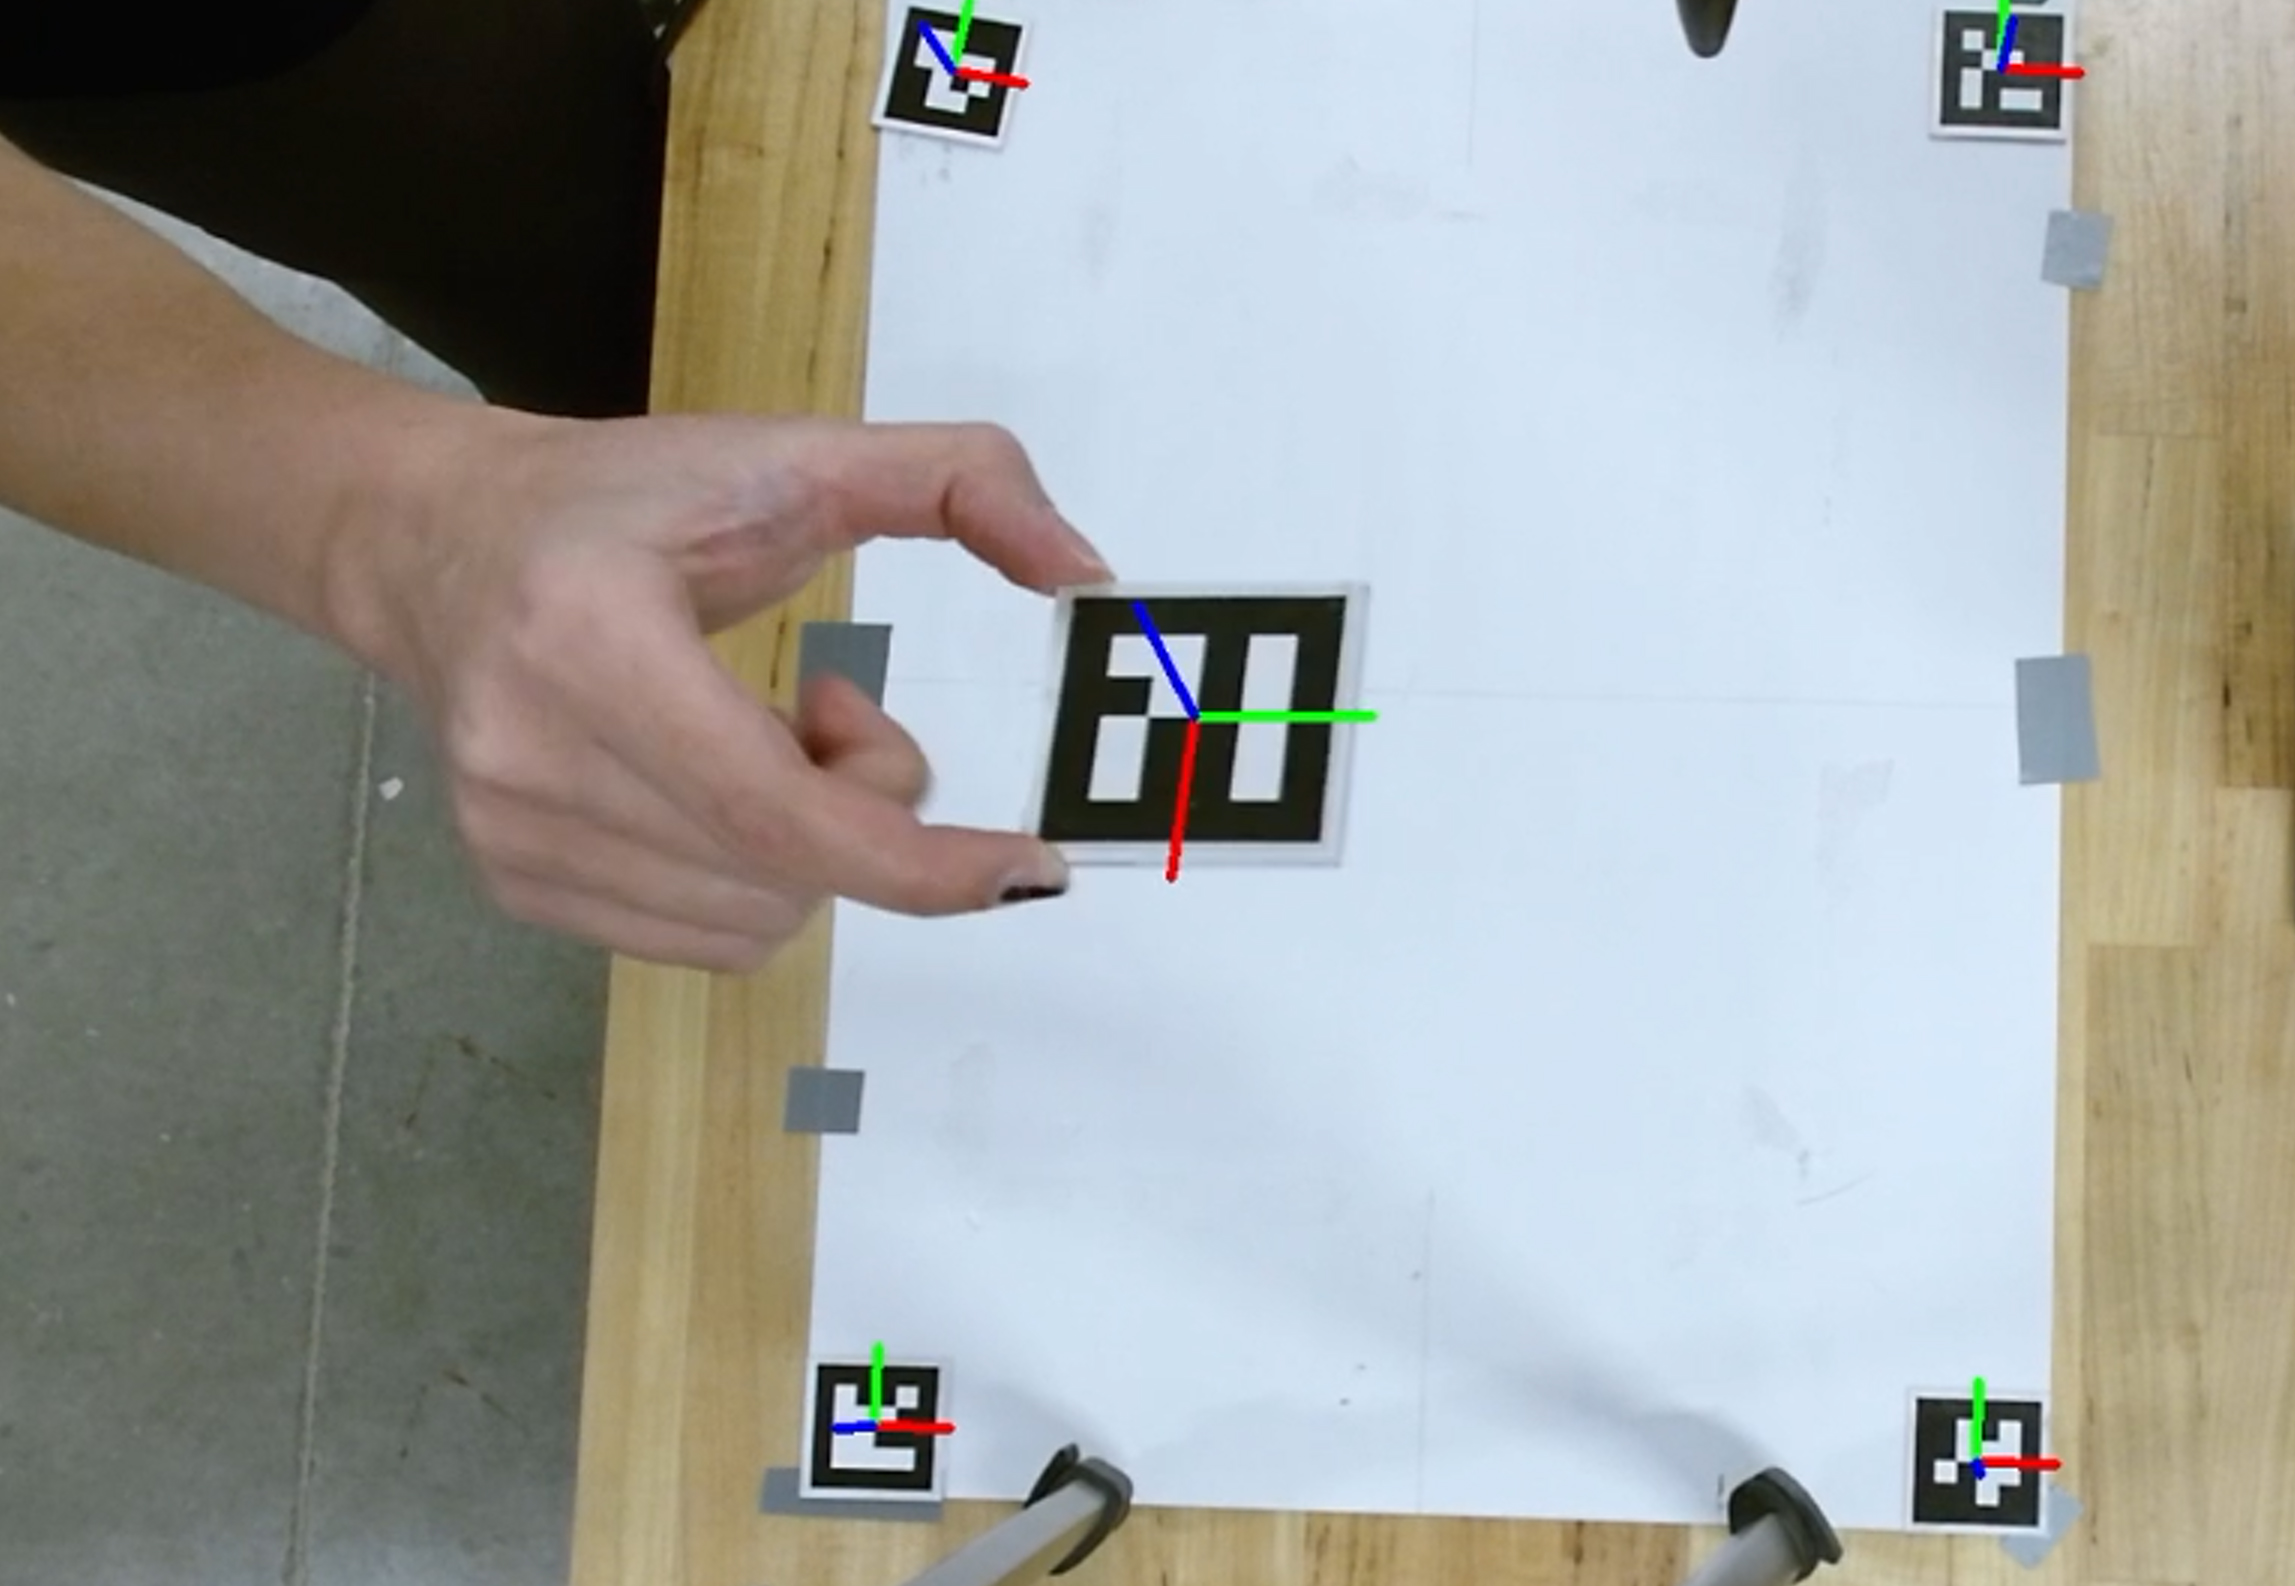
\includegraphics[width=0.8\textwidth]{pictures/tracking_aruco.jpg}
            \caption{Real-Time Tracking with ArUco}
            \label{fig:imagen2}
        \end{minipage}
        \caption{Common applications of ArUco markers.}
    \end{figure}

    \subsubsection{Marker Formats}

    ArUco markers consist of an outer black border and an internal region encoding a unique binary pattern. Depending on the dictionary being used, the number of bits in the marker varies, affecting the likelihood of confusion with other markers and the detection distance. A higher resolution allows markers to be detected from greater distances but may require more processing \cite{aruco_docs}.

    The ArUco library also supports creating custom dictionaries, allowing developers to adapt markers to the specific needs of their projects. \textit{“The design of a dictionary is important since the idea is that their markers should be as different as possible to avoid confusions”} \cite{aruco_docs_pdf}. This flexibility is especially useful in projects where ensuring the uniqueness and reliability of marker detection in complex environments is crucial.

    \begin{figure}[h!] 
    \centering 
    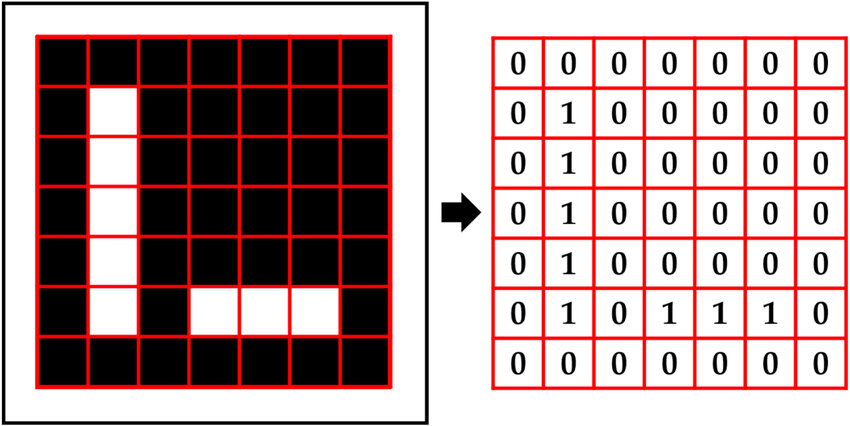
\includegraphics[width=0.8\textwidth]{pictures/bits_aruco.png} % Example of an ArUco marker with its binary format 
    \caption{Bits of a 7x7 ArUco marker.} 
    \label{fig} 
    \end{figure}

\subsection{Aruco vs. Embedded Aruco}

    ArUco markers and Embedded ArUco markers (e-ArUco) are technologies used in computer vision for detection and pose estimation tasks. While they share a common basis in their design and detection algorithms, they have significant differences that make them suitable for different applications, particularly in high-precision operations.

    \subsubsection{Key Differences}

    The main difference between traditional ArUco markers and Embedded ArUco markers lies in the latter's optimization for high-precision detection over a wide range of distances. According to Khazetdinov et al. (2021), \textit{“a new type of fiducial marker called embedded ArUco (e-ArUco) was developed specially for a task of robust marker detection for a wide range of distances”} \cite{khazetdinov2021}. e-ArUco markers are designed to maintain detectability and precision in scenarios where standard ArUco markers might not perform as effectively, such as when millimeter-level accuracy is required in UAV landing applications.

    Another significant difference is that e-ArUco markers are designed to improve detection robustness, minimizing errors that could arise from changing lighting conditions and partial occlusions. These markers build upon ArUco detection algorithms, allowing implementation without substantial changes to existing ArUco-based systems \cite{khazetdinov2021}.

    \begin{figure}[h!]
        \centering
        \begin{minipage}{0.3\textwidth}
            \centering
            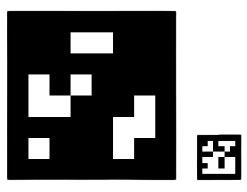
\includegraphics[width=0.65\textwidth]{pictures/pose_1.png}
            \caption{Large/Small ArUco Marker Generation.}
            \label{fig:imagen1}
        \end{minipage}
        \hfill
        \begin{minipage}{0.3\textwidth}
            \centering
            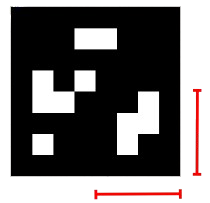
\includegraphics[width=0.55\textwidth]{pictures/pose_2.png}
            \caption{Calculating the Large ArUco Marker Center.}
            \label{fig:imagen2}
        \end{minipage}
        \hfill
        \begin{minipage}{0.3\textwidth}
            \centering
            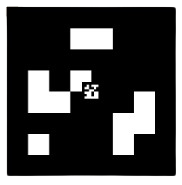
\includegraphics[width=0.5\textwidth]{pictures/pose_3.png}
            \caption{Overlaying the Small ArUco Marker on the Large Center.}
            \label{fig:imagen2}
        \end{minipage}
        \caption{Generation process of e-ArUco markers.}
    \end{figure}

    \subsubsection{Use Cases}

    Traditional ArUco markers, as mentioned in the previous section, are commonly used in applications such as augmented reality, pose estimation, and robot and drone navigation. These markers are versatile and adaptable to various applications that do not require extreme precision, making them ideal for localization, augmented reality, etc.

    On the other hand, Embedded ArUco markers (e-ArUco) are specifically designed for scenarios where higher precision is critical. A notable example is their use in UAV (Unmanned Aerial Vehicle) landing, where precise and reliable detection is needed across different distances. In a study by Khazetdinov et al., \textit{“an average landing accuracy was 2.03 cm with a standard deviation of 1.53 cm”} was achieved using e-ArUco markers and a landing algorithm implemented in ROS and tested in the Gazebo simulator \cite{khazetdinov2021}. This capability makes e-ArUco markers ideal for environments requiring millimeter-level precision, such as in high-precision autonomous landing operations.

\subsection{Aruco Detection}
    ArUco marker detection is an essential process in computer vision that enables the identification and pose estimation of markers in images. The following section details detection algorithms, OpenCV implementation, and parameters that affect detection accuracy.

    \subsubsection{Detection Algorithms}

    ArUco marker detection relies on computer vision algorithms that identify contours and specific patterns in images. According to OpenCV documentation, the detection process begins by identifying squares in the image and verifying if they contain a valid binary pattern corresponding to an ArUco marker \cite{opencv_docs_aruco}. The algorithm implemented in OpenCV uses contour segmentation and edge detection to find square regions, which are then checked to determine if they match the patterns in the ArUco dictionary.

    Once a marker is identified, the algorithm calculates the camera's pose relative to the marker using inverse projection. This process is particularly important in applications requiring the calculation of the camera's position and orientation for robot and drone navigation and control.

    \subsubsection{OpenCV Implementation}

    OpenCV provides a robust implementation for detecting ArUco markers through the \texttt{cv::aruco} module. The main function for detection is \texttt{cv::aruco::detectMarkers}, which identifies markers in an image and returns their corners and corresponding IDs. OpenCV documentation highlights that \textit{“the function detects the markers and returns their IDs and corner positions in the image”} \cite{opencv_tutorial_aruco}.

    The following example demonstrates how to use OpenCV to detect ArUco markers in Python:

    \begin{verbatim}
    import cv2
    import cv2.aruco as aruco

    # Load the image
    image = cv2.imread('image_path.jpg')

    # Define the ArUco dictionary
    aruco_dict = aruco.Dictionary_get(aruco.DICT_6X6_250)

    # Detect markers
    corners, ids, _ = aruco.detectMarkers(image, aruco_dict)

    # Draw detected markers
    if ids is not None:
        aruco.drawDetectedMarkers(image, corners, ids)
    \end{verbatim}

    After obtaining the corners and IDs of the markers, this information can be used to calculate the camera's pose relative to the detected marker(s). To calculate the center of an ArUco marker, the detected corners and marker size can be used to estimate its position in the image.

    \subsubsection{Accuracy Parameters}

    The accuracy of ArUco marker detection depends on several factors, including image quality, marker size, and camera calibration parameters. According to OpenCV documentation, precise camera calibration is crucial to minimize errors in pose estimation \cite{opencv_docs_aruco}. Key parameters affecting detection include:

    \begin{itemize}
        \item \textbf{Lens distortion}: Correcting lens distortion improves detection accuracy.
        \item \textbf{Marker resolution}: Higher-resolution markers allow for more accurate detection at greater distances but require more processing power.
        \item \textbf{Lighting and contrast}: Detection can be affected by varying lighting conditions, so it is important for the image to have good contrast between the marker and the background.
    \end{itemize}

    \begin{figure}[h!] 
        \centering 
            \begin{minipage}{0.48\textwidth}
                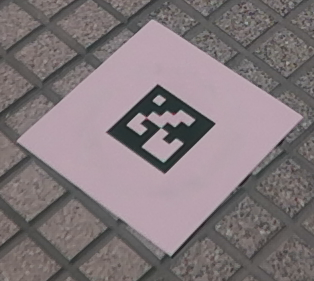
\includegraphics[width=0.8\textwidth]{pictures/aruco_no_pose_estimation.png} % Example of ArUco markers 
                \caption{ArUco without pose estimation.} 
                \label{fig:aruco_no_pose_estimation}
            \end{minipage}
            \begin{minipage}{0.48\textwidth}
                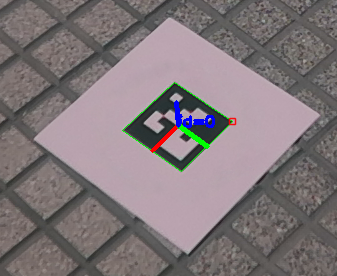
\includegraphics[width=0.8\textwidth]{pictures/aruco_pose_estimation.png} % Example of ArUco markers 
                \caption{ArUco with pose estimation.} 
                \label{fig:aruco_pose_estimation}
            \end{minipage}
    \end{figure}

\subsection{ROS2-Pixhawk Communication}
    Communication between ROS 2 and Pixhawk is based on the MAVLink protocol, a lightweight protocol that enables bidirectional data transfer between the flight controller and a companion computer. This integration is critical for sending real-time flight commands and monitoring the drone's status.
    
        \subsubsection{MAVLink Protocol}
        MAVLink (Micro Air Vehicle Link) is a high-performance communication protocol designed for unmanned vehicle systems. According to the official documentation, \textit{“MAVLink is a very lightweight, header-only message marshalling library for micro air vehicles”} \cite{mavlink_docs}. This protocol uses a message-based packet system that facilitates data transmission between the ground control station and the unmanned vehicle.

        MAVLink messages are structured into specific commands that control various aspects of flight and telemetry, including parameters such as position, speed, battery status, and flight control commands. Each message is identified by a unique ID, which simplifies processing and enables efficient real-time communication.

        \subsubsection{MAVLink Integration Options in ROS 2}
        To facilitate MAVLink integration with ROS 2, several communication options exist for sending and receiving data between a companion computer and the Pixhawk flight controller. The two most popular solutions are MAVROS and Micro XRCE-DDS.

            \paragraph{MAVROS}
            MAVROS is a set of ROS nodes that act as an interface between ROS and MAVLink, allowing ROS to communicate with the flight controller through topics and services. MAVROS enables the publication and subscription of MAVLink messages via ROS topics, facilitating flight command execution, telemetry data retrieval, and mission control.

            MAVROS implements a series of predefined ROS topics, such as:
            \begin{itemize}
                \item \texttt{/mavros/setpoint\_position/local}: To set position waypoints.
                \item \texttt{/mavros/state}: Provides the current state of the drone, including the flight mode and whether the vehicle is armed.
                \item \texttt{/mavros/imu/data}: IMU data for monitoring orientation and acceleration.
                \item \texttt{/mavros/battery}: Displays battery data, such as charge percentage and voltage.
            \end{itemize}
            
            With MAVROS, developers can send control commands, such as arming the drone, changing flight modes, or setting waypoints for autonomous navigation. This is achieved by publishing messages to the appropriate topics and adjusting parameters in real-time via the MAVLink interface \cite{px4_ros2}.
            
            \begin{figure}
                \centering
                %\includegraphics[width=0.8\textwidth]{pictures/mavros.png} 
                %\caption{ROS 2 - Pixhawk communication using MAVROS.}
                \label{fig:mavros}
            \end{figure}

            \paragraph{Micro XRCE-DDS}
            Micro XRCE-DDS is a lightweight implementation of DDS (Data Distribution Service) that allows efficient communication between ROS 2 and the flight controller in systems with resource constraints. This option is useful in contexts where system size and performance are critical, such as small drones or those with limited processing hardware.
    
            With Micro XRCE-DDS, ROS 2 can directly communicate with PX4 using the DDS middleware. This enables the creation of a distributed and scalable system, where ROS 2 nodes can send and receive MAVLink messages via DDS topics, similar to MAVROS but with optimized processing overhead \cite{px4_ros2}.
    
            \begin{figure}
                \centering
                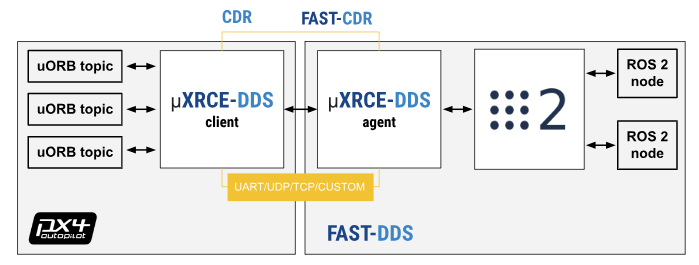
\includegraphics[width=0.8\textwidth]{pictures/xrce_dds.png} 
                \caption{ROS 2 - Pixhawk communication using Micro XRCE-DDS.}
                \label{fig:xrce_dds}
            \end{figure}

    
\subsection{Sensors for Navigation in Outdoor and Indoor Environments}
To achieve precise control of the drone's position using ROS 2 topics such as Òtexture{/mavros/setpoint/position/local}, it is necessary to have sensors that provide reliable positioning data depending on the environment in which the drone is operating. Sensors commonly used in outdoor and indoor environments to provide position information are described below.    
    \subsubsection{Outdoor Environment Sensors}
    In outdoor environments, drones often use global positioning sensors (GPS) to determine their location in real time. The following are the most common outdoor sensors:
    \begin{itemize}
        \item \textbf{GPS (Global Positioning System):} GPS is the primary sensor for outdoor navigation. It provides latitude, longitude, and altitude coordinates that allow the drone to determine its global position. In ROS 2, this data is usually published in topics such as \texttt{/mavros/global\_position/global} and integrated into the position control systems \cite{gps_reference}.
        \item \textbf{RTK-GPS (Real-Time Kinematic GPS):} For high-precision applications, such as precision landing or navigation in restricted areas, RTK-GPS is used. This system improves the accuracy of GPS by correcting data in real time, reaching centimeter accuracies. RTK-GPS is compatible with MAVLink and enables highly accurate position control in ROS 2 \cite{gps_reference}.
        \item \textbf{IMU (Inertial Measurement Unit):} Besides it does not provide direct location data, the IMU complements GPS by detecting changes in orientation and acceleration. This data is crucial for maintaining stability and providing information about the drone's orientation during flight \cite{gps_reference}.
    \end{itemize}
    
    \subsubsection{Sensors for Indoor Environments}
    In indoor environments, where GPS signals are often weak or non-existent, other sensors are used to determine the drone's position and navigation. Sensors used indoors include:
    \begin{itemize}
        \item \textbf{Vision Cameras (Monocular or Stereo):} Vision cameras allow visual localization using SLAM (Simultaneous Localization and Mapping) algorithms or marker detection, such as ArUco, to calculate the relative position of the drone indoors. With ROS 2, these cameras can be integrated with libraries such as OpenCV and use the image topics for real-time processing \cite{non_gps_navigation}.
    
        \item \textbf{LIDAR (Light Detection and Ranging):} LIDAR sensors emit pulses of light to measure distances and obtain detailed maps of the environment. These sensors are useful for real-time indoor navigation and mapping and are integrated into ROS 2 using point cloud topics. They are particularly effective for obstacle avoidance and precise indoor positioning \cite{non_gps_navigation}.
        
        \item \textbf{Vicon Motion Capture System:} Vicon cameras are a high-precision motion capture system that utilize multiple cameras placed around a testing environment to track reflective markers attached to the drone. By triangulating the position of these markers, the Vicon system provides accurate 3D position and orientation data. This data can be used in ROS 2 for real-time drone control and navigation, typically by publishing the position data as a topic. The Vicon system is ideal for precise indoor positioning, particularly in controlled environments where high accuracy is required \cite{non_gps_navigation}.

        \item \textbf{IMU (Inertial Measurement Unit):} Indoors, the IMU remains an essential component for detecting changes in orientation and motion. Fusion of IMU data with other sensors, such as LIDAR or cameras, helps maintain stability and provides accurate position estimates using fusion filters, such as the Kalman filter \cite{non_gps_navigation}.
        
    \end{itemize}
    
    

